\documentclass[aspectratio=169,9pt]{beamer}

\usepackage[utf8]{inputenc}
\usepackage{graphicx}
\graphicspath{ {./figures/} }
\usepackage{caption}
\usepackage{subcaption}
% \captionsetup{font=tiny,labelfont=tiny}
\usepackage{hyperref}
\usepackage{amsmath}
\usepackage{tikz}
\usepackage[strict]{changepage}
\usetikzlibrary{arrows,automata,positioning}
\usetheme[titleformat=smallcaps,
			sectionpage=progressbar,
			subsectionpage=progressbar,
			progressbar=frametitle,
			numbering=fraction]{metropolis}
\usecolortheme{owl}
\usepackage[style=apa,
			sorting=nyt,
			date=year,
			bibencoding=utf8,
			isbn=false,
			eprint=false,
			dashed=false,
			uniquelist=false,
			maxbibnames=10,
			minbibnames=1,
			maxcitenames=2,
			uniquename=init,
			giveninits=true,
			useprefix=false,
			minsortnames=1,
			maxsortnames=2]{biblatex}
  \bibliography{References}
% Information to be included in the title page:
\title{Markovian modelling of allelic coordination of transcriptional bursting}
\author{Harshavardhan BV}
\date{\today}
\institute{IISc Bangalore}

\begin{document}
\frame{\titlepage}

\section{Introduction}
\begin{frame}{What are alleles?}
  \begin{figure}
    \includegraphics[width=\textwidth]{allele}
    \caption{Schematic figure of Allele}
  \end{figure}
 \pause Copies of the same gene on two chromosomes
\end{frame}

\begin{frame}{How do the alleles express?}
  \begin{figure}
    \centering
    \includegraphics[width=0.8\textwidth]{allelic}
    \caption{Allelic expression types}
  \end{figure}
  \begin{itemize}
    \item \pause Imprinted vs Random
    \item \pause Fixed vs Dynamic \pause $\leftarrow$ Stochastic bursting
  \end{itemize}
  \footcite{Singer2010}
\end{frame}

\begin{frame}{How to coordinate?}
  \begin{itemize}
    \item $p_0$ = probability of both alleles off
    \item $p_2$ = probability of both alleles on
    \item \pause Fully coordinated - both off $	\longleftrightarrow$ both on
    $$p_{0} + p_{2} = 1$$
    \item \pause Fully independent 
    $$p = \text{probability of 1 gene being on}$$
    $$p_2 = p^2 \quad ; \quad p_0 = (1-p)^2$$
    $$\sqrt{p_0} + \sqrt{p_2} = 1$$
  \end{itemize} 
  \footcite{Naik2021}
\end{frame}

\begin{frame}{Existing Work}
  Alleles are semi-coordinated in developmental genes
  \begin{columns}
    \begin{column}{0.63\textwidth}
      \begin{figure}
        \centering
        \includegraphics[width=\textwidth]{hemant}
        \caption{Experimental Data}
      \end{figure}
    \end{column}
    \begin{column}{0.33\textwidth}
      \begin{figure}
        \centering
        \includegraphics[width=\textwidth]{kishore}
        \caption{Kishore's Model}
      \end{figure}
    \end{column}
  \end{columns}
\footnote{Images from: \cite{Naik2021}}
\end{frame}

\begin{frame}{Context for cancer?}
  \begin{itemize}
    \item Introduces non-genetic heterogeneity
    \begin{itemize}
      \item Switch between alleles 
      \item Modulate dosage levels
    \end{itemize}
    \item \pause Coordinated bursts $\leftarrow$ therapy resistance \parencite{Schuh2020}
  \end{itemize}
\end{frame}

\section{Modelling}

\begin{frame}{Markov Model}
    \begin{columns}
        \begin{column}{0.65\textwidth}
            \begin{figure}
                \centering
                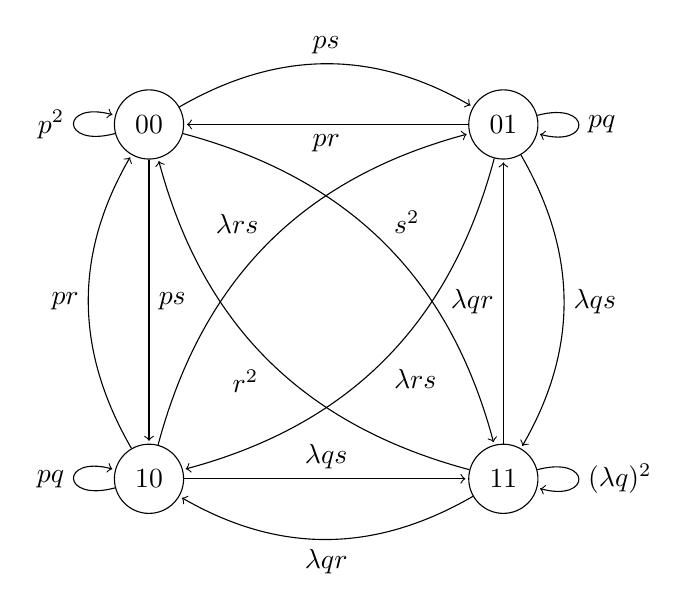
\begin{tikzpicture}[shorten >=1pt,node distance=4.5cm and 1cm,on grid,auto]
                    \node[state] (00)  {$00$};
                    \node[state] (01) [right of=00]  {$01$};
                    \node[state] (10) [below of=00] {$10$};
                    \node[state] (11) [below of=01] {$11$}; 
                    \path[->]
                        (00) edge [loop left] node {$p^2$}    ()
                            edge [bend left]  node {$ps$}    (01)
                            edge node {$ps$}    (10)
                            edge [bend left] node {$s^2$}    (11)
                        (01) edge [loop right] node {$pq$}    ()
                            edge node {$pr$}    (00)
                            edge [bend left] node {$\lambda rs$}    (10)
                            edge [bend left] node {$\lambda qs$}    (11)
                        (10) edge [loop left] node {$pq$}    ()
                            edge [bend left] node {$pr$}    (00)
                            edge [bend left] node {$\lambda rs$}    (01)
                            edge node {$\lambda qs$}    (11)
                        (11) edge [loop right] node {$(\lambda q)^2$}    ()
                            edge [bend left] node {$r^2$}    (00)
                            edge node {$\lambda qr$}    (01)
                            edge [bend left] node {$\lambda qr$}    (10);
                \end{tikzpicture}
                \caption{Markov State Diagram}
            \end{figure} 
        \end{column}
        \begin{column}{0.35\textwidth}
        Where,
            \begin{itemize}
                \item 0 $\implies$ Gene Off
                \item 1 $\implies$ Gene On
                \item \pause $p$ = StayOff rate
                \item $q$ = StayOn rate
                \item $r$ = Off rate
                \item $s$ = On rate
                \item $\lambda$ = Interaction Parameter
            \end{itemize}
        \end{column}
    \end{columns}
\end{frame}

\begin{frame}{Transition Matrix}
  \begin{columns}
    \begin{column}{0.6\textwidth}
      \[ T =
      \begin{bmatrix}
              p^2 & pr & pr & r^2 \\
              ps & pq & \lambda rs & \lambda qr \\
              ps & \lambda rs & pq & \lambda qr \\
              s^2 & \lambda qs & \lambda qs & (\lambda q)^2 \\
      \end{bmatrix}
      \]
      \begin{figure}
        \centering
        \includegraphics[width=0.4\textwidth]{matrix_meme}
        \caption{We live in a matrix (meme)}
      \end{figure}
    \end{column}
    \begin{column}{0.4\textwidth}
      \pause
      At steady state
      $$ T\vec{E} = 1 \vec{E}$$
      $$ \vec{E} = \begin{bmatrix}p_{00} \\ p_{01} \\ p_{10} \\ p_{11} \end{bmatrix}$$
      \begin{itemize}
        \item $\sum_j T_{ij} = 1 \quad \forall i$
        \item $E_i \implies$  P(state=i)
        \item $\sum_i E_{i} = 1$
      \end{itemize}
    \end{column}
  \end{columns}
\end{frame}

\section{Preliminary Results}

\begin{frame}{Random Sampling}
  \begin{figure}[h]
      \begin{adjustwidth}{-5cm}{-5cm}
        \centering
        \begin{subfigure}[b]{0.33\textwidth}
          \centering
          \includegraphics[width=\textwidth]{loguni-p2vp0-classified.pdf}
          \caption{$p_2$ vs $p_0$}
        \end{subfigure}\pause
        \begin{subfigure}[b]{0.66\textwidth}
          \centering
          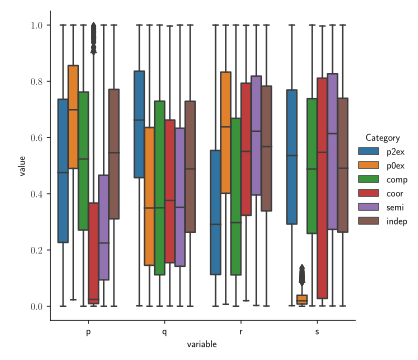
\includegraphics[width=\textwidth]{loguni-parms.pdf}
          \caption{Parameters}
        \end{subfigure}
      \end{adjustwidth}
      \pause[-1]\caption{ $p,q,r,s \in U[0,1]$, $\lambda$ sampled log-uniformly $\in [0.01,100]$}
    \end{figure}
\end{frame}

\begin{frame}{Parameter sweep}
  \begin{figure}[h]
    \begin{adjustwidth}{-7cm}{-7cm}
      \centering
      \begin{subfigure}[b]{0.2\textwidth}
        \centering
        \includegraphics[width=\textwidth]{sweep-p}
        \caption{$p$}
      \end{subfigure}\pause
      \begin{subfigure}[b]{0.2\textwidth}
        \centering
        \includegraphics[width=\textwidth]{sweep-q}
        \caption{$q$}
      \end{subfigure}\pause
      \begin{subfigure}[b]{0.2\textwidth}
        \centering
        \includegraphics[width=\textwidth]{sweep-r}
        \caption{$r$}
      \end{subfigure}\pause
      \begin{subfigure}[b]{0.2\textwidth}
        \centering
        \includegraphics[width=\textwidth]{sweep-s}
        \caption{$s$}
      \end{subfigure}\pause
      \begin{subfigure}[b]{0.2\textwidth}
        \centering
        \includegraphics[width=\textwidth]{sweep-l}
        \caption{$\lambda$}
      \end{subfigure}
    \end{adjustwidth}
    \pause[-1]\caption{Parameter sweep}
  \end{figure}
  \footnote{$\lambda$ labels in $log_{10}$}
\end{frame}

\begin{frame}{Paired Parameter sweep}
  \begin{figure}[h]
    \begin{adjustwidth}{-7cm}{-7cm}
      \centering
      \begin{subfigure}[b]{0.25\textwidth}
        \centering
        \includegraphics[width=\textwidth]{sweep-sl-l}
        \caption{$s \& \lambda$ with $\lambda$ coloured}
      \end{subfigure}
      \begin{subfigure}[b]{0.25\textwidth}
        \centering
        \includegraphics[width=\textwidth]{sweep-sl-s}
        \caption{$s \& \lambda$ with $s$ coloured}
      \end{subfigure}\pause
      \begin{subfigure}[b]{0.25\textwidth}
        \centering
        \includegraphics[width=\textwidth]{sweep-rl-l}
        \caption{$r \& \lambda$ with $\lambda$ coloured}
      \end{subfigure}
      \begin{subfigure}[b]{0.25\textwidth}
        \centering
        \includegraphics[width=\textwidth]{sweep-rl-r}
        \caption{$r \& \lambda$ with $r$ coloured}
      \end{subfigure}
    \end{adjustwidth}
    \pause[-1]\caption{Parameter sweep in pairs}
  \end{figure}
  \footnote{$\lambda$ labels in $log_{10}$}
\end{frame}

\begin{frame}{Paired Parameter sweep}
  \begin{figure}[h]
    \begin{adjustwidth}{-7cm}{-7cm}
      \centering
      \begin{subfigure}[b]{0.25\textwidth}
        \centering
        \includegraphics[width=\textwidth]{sweep-pl-l}
        \caption{$p \& \lambda$ with $\lambda$ coloured}
      \end{subfigure}
      \begin{subfigure}[b]{0.25\textwidth}
        \centering
        \includegraphics[width=\textwidth]{sweep-pl-p}
        \caption{$p \& \lambda$ with $p$ coloured}
      \end{subfigure}\pause
      \begin{subfigure}[b]{0.25\textwidth}
        \centering
        \includegraphics[width=\textwidth]{sweep-ql-l}
        \caption{$q \& \lambda$ with $\lambda$ coloured}
      \end{subfigure}
      \begin{subfigure}[b]{0.25\textwidth}
        \centering
        \includegraphics[width=\textwidth]{sweep-ql-q}
        \caption{$q \& \lambda$ with $q$ coloured}
      \end{subfigure}
    \end{adjustwidth}
    \pause[-1]\caption{Parameter sweep in pairs}
  \end{figure}
  \footnote{$\lambda$ labels in $log_{10}$}
\end{frame}

\section{Conclusions?}
\begin{frame}{Why this model?}
  \begin{itemize}
    \item \pause Kishore's model is ``more complicated"
    \item \pause Discrete nature of transcriptional activity$^*$
    \item \pause Inherently stochastic
    \item \pause Can do both steady state and dynamic analysis
  \end{itemize}
\end{frame}

\begin{frame}{Assumptions and Caveats}
  \begin{itemize}
    \item \pause[2] Redundancy: $[0.5,0.5,0.5,0.5,1.0] \equiv [1.0,1.0,1.0,1.0,1.0]$
    \item \pause[2] Difficult to understand parameters
    \item Alleles symmetric - same gene
    \item \pause Mechanism of Interaction/Influence unknown
    \item \pause Instantaneous interaction (no memory)
    \item \pause Might not account for some biological phenomena (Eg: Gene more likely to stay On if On, and vice-versa)
    \item \pause Not tested on cancer systems
  \end{itemize}
\end{frame}

\begin{frame}[standout]
  Thank You

  Questions, Comments, Feedback
\end{frame}

\begin{frame}[allowframebreaks]
  \printbibliography
\end{frame}

\end{document}